\section{Requisiti Funzionali}
In questo capitolo vengono ripresi i requisiti funzionali precedentemente descritti in linguaggio naturale e vengono riscritti in linguaggio formale UML use-case diagram. Si va inoltre più nello specifico, mostrando quali attori sono coinvolti in ciascuna funzione e illustrando il ruolo che svolgono all'interno di essa.

\subsection{Compendio degli alfabeti} \label{req_compendio_alfabeti}
\begin{figure}[!h]
\centering
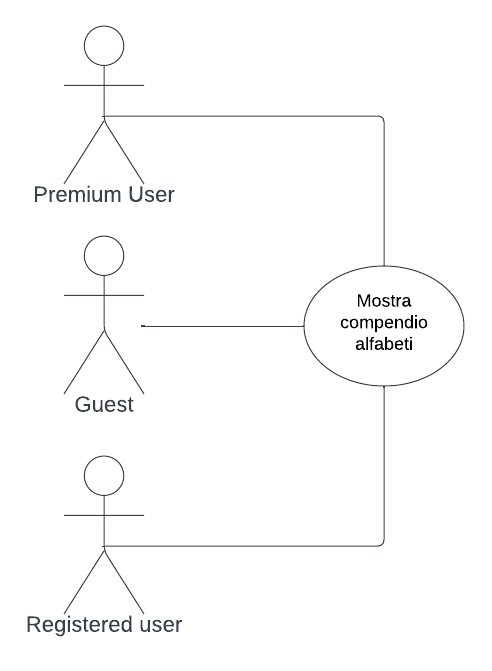
\includegraphics[scale=0.35]{images/use_case_compendio.png}
\end{figure}
\noindent
\textbf{Titolo}: mostrare compendio alfabeti \\
\\
\textbf{Riassunto}: questo use-case spiega come i diversi tipi di utenti possono accedere al compendio degli alfabeti. \\
\\
\textbf{Descrizione}:
\begin{enumerate}
    \item L'utente, che sia autenticato o non autenticato che si trova nella pagina principale dell'applicazione, clicca sul pulsante 'info'.
    \item Il sistema porterà l'utente in una nuova pagina in cui gli sarà mostrata una descrizione dei tre alfabeti utilizzati per la nostra applicazione. Oltre a ciò gli saranno resi disponibili due tabelle e una lista. Le tabelle conterranno tutti i simboli degli alfabeti Hiragana e Katakana, mentre la lista conterrà tutti i simboli dell'alfabeto Kanji che sono stati utilizzati, specificatamente all'interno dell'applicazione.
\end{enumerate}

\newpage
\subsection{Registrazione} \label{req_registrazione}

\begin{figure}[!h]
\centering
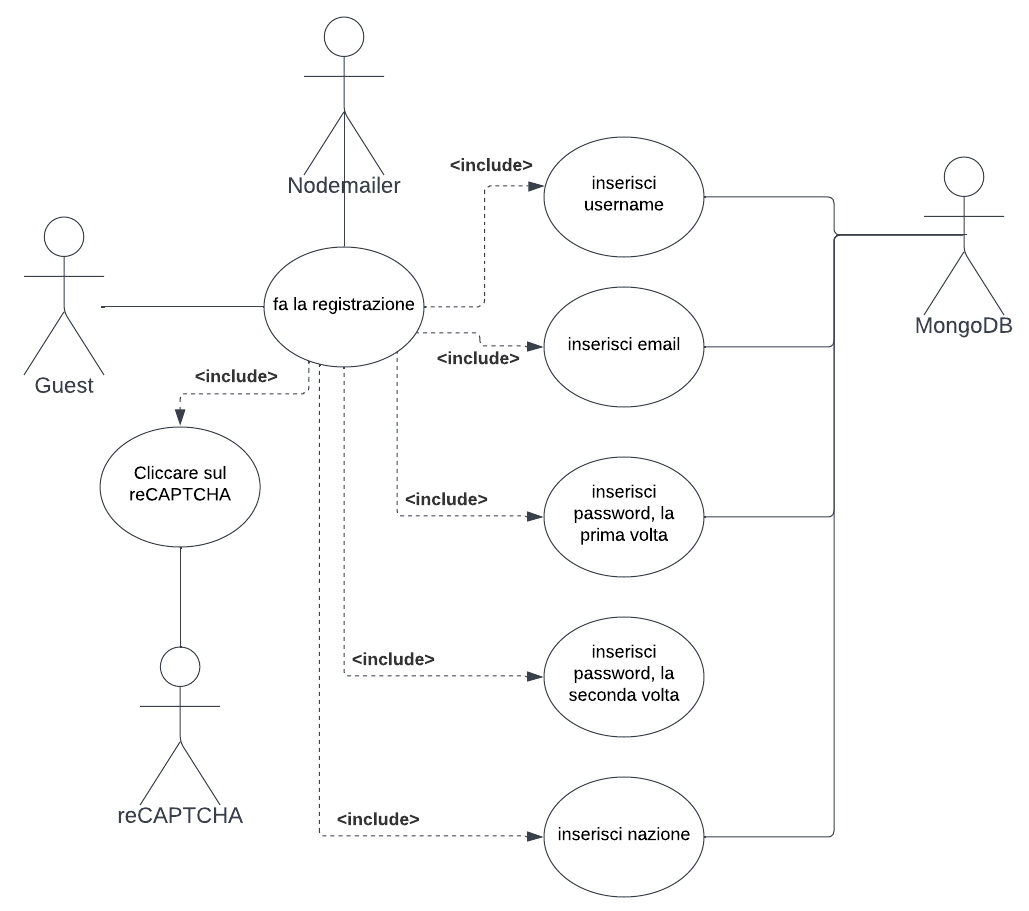
\includegraphics[scale=0.35]{images/use_case_registrazione.png}
\end{figure}
\noindent
\textbf{Titolo}: registrazione \\
\\
\textbf{Riassunto}: questo use-case spiega come un utente anonimo (guest), può registrarsi. \\
\\
\textbf{Descrizione}:
\begin{enumerate}
    \item L'utente che si trova nella pagina di registrazione, inserisce in degli appositi campi le seguenti informazioni: username, e-mail, password, conferma password e nazione.
    \item L'utente clicca sul reCAPTCHA e poi sul pulsante 'create account', per confermare che si tratta di un essere umano e per confermare i dati precedentemente inseriti. {[ Eccezione 1 ]}
    \item Il sistema attraverso delle chiamate al database MongoDB, memorizza username, e-mail, password e nazione, come un nuovo utente. {[ Eccezione 2 ]}
    \item L'applicazione invia all’utente un’e-mail di conferma dell’avvenuta registrazione. {[ Eccezione 3 ]}
    \item L'utente è finalmente stato registrato e ritorna alla pagina principale dell'applicazione, con login già effettuato. 
\end{enumerate}
\textbf{Eccezioni}: \\
{[ Eccezione 1 ]} nel caso in cui l'utente si è dimenticato di inserire qualche campo, di cliccare sul reCAPTCHA, i campi password e conferma password non coincidono, allora un messaggio di errore viene mostrato a video. \\
{[ Eccezione 2 ]} nel caso in cui esista già un utente con quello specifico username o e-mail, non si procede e sarà visualizzato un messaggio di errore. \\
{[ Eccezione 3 ]} l'e-mail inserita non esiste e allora viene stampato a video un messaggio di errore. 

\subsection{Login con credenziali} \label{req_login_con_credenziali}
\begin{figure}[!h]
\centering
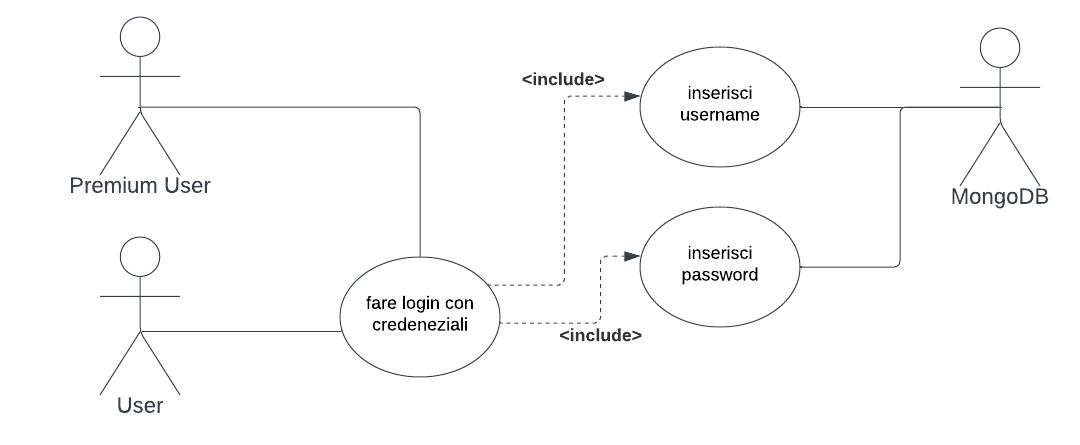
\includegraphics[scale=0.35]{images/use_case_login_con_credenziali.png}
\end{figure}
\noindent
\textbf{Titolo}: login con credenziali \\
\\
\textbf{Riassunto}: questo use-case spiega come un utente registrato o di livello superiore, può fare il login all'interno dell'applicazione usando le credenziali inserite nella fase di registrazione. \\
\\
\textbf{Descrizione}:
\begin{enumerate}
    \item L'utente che si trova nella pagina di login, inserisce l'username e la password relativi al proprio account e clicca sul pulsante 'login'.
    \item L'applicazione interagisce con il sistema esterno MongoDB, per verificare che le credenziali inserite siano valide. {[ Eccezione 1 ]}
    \item Viene eseguito il login e viene fatto ritornare l'utente alla pagina principale dell'applicazione.
\end{enumerate}
\textbf{Eccezioni}: \\
{[ Eccezione 1 ]} se l'username inserito non esiste oppure la password non è corretta, non si procede e sarà visualizzato un messaggio all'utente con scritto username o password errata.
\newpage

\subsection{Login con google} \label{req_login_con_google}
\begin{figure}[!h]
\centering
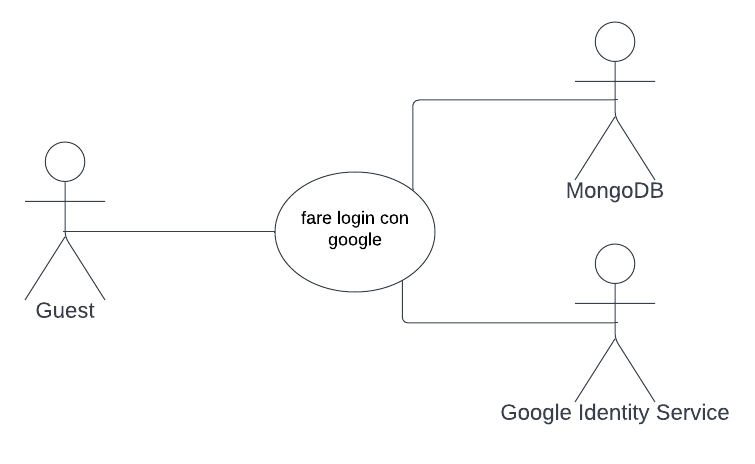
\includegraphics[scale=0.35]{images/use_case_login_con_google.png}
\end{figure}
\noindent
\textbf{Titolo}: login con google \\
\\
\textbf{Riassunto}: questo use-case spiega come un utente non registrato, può fare il login all'interno dell'applicazione usando il proprio account google. \\
\\
\textbf{Descrizione}:
\begin{enumerate}
    \item L'utente che si trova nella pagina di login, clicca sul pulsante che gli permetterà di effettuare il login con google.
    \item L'applicazione grazie alle API di google interagirà con il Google Identity Service e si aprirà una finestra che permetterà all'utente di effettuare il login tramite credenziali (e-mail e password) di google. 
    \item Dopo che l'utente avrà effettuato l'autenticazione con le proprie credenziali google, il sistema interagirà con il database MongoDB per creare un entry all'interno database, nel caso in cui non fosse già presente, per ricordarsi che l'utente si è registrato/loggato con account google.
    \item Viene fatto ritornare l'utente alla pagina principale dell'applicazione.
\end{enumerate}

\newpage
\subsection{Logout} \label{req_login_logout}
\begin{figure}[!h]
\centering
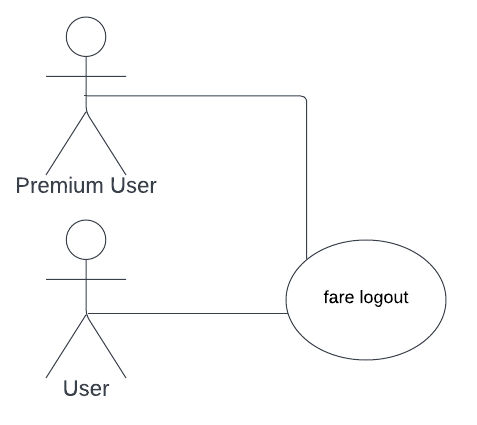
\includegraphics[scale=0.35]{images/use_case_logout.png}
\end{figure}
\noindent
\textbf{Titolo}: logout dall'applicazione \\
\\
\textbf{Riassunto}: questo use-case spiega come un utente registrato o di livello superiore può uscire dal proprio account. \\
\\
\textbf{Descrizione}:
\begin{enumerate}
    \item L'utente che si trova nella pagina di principale dell'applicazione, clicca sul icona del proprio profilo e seleziona la voce 'logout'.
    \item Il sistema fa uscire l'utente dal proprio profilo e lo trasferisce nella pagina principale come utente guest.
\end{enumerate}

\subsection{Visualizzazione dati personali} \label{req_visualizzazione_dati_personali}
\begin{figure}[!h]
\centering
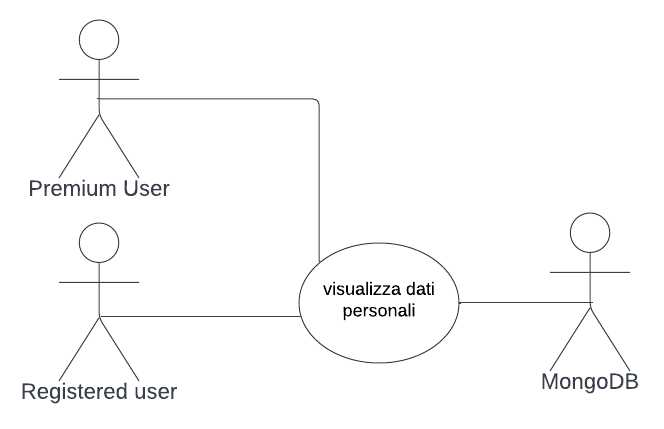
\includegraphics[scale=0.35]{images/use_case_visualizza_dati_personali.png}
\end{figure}
\noindent
\textbf{Titolo}: visualizzazione dati personali \\
\\
\textbf{Riassunto}: questo use-case mostra come un utente registrato o di livello superiore può visualizzare i propri dati personali inseriti in fase di registrazione. \\
\\
\textbf{Descrizione}:
\begin{enumerate}
    \item L'utente che si trova nella pagina principale dell'applicazione, clicca sul icona del proprio profilo e seleziona la voce 'my account'.
    \item L'applicazione interagirà con il sistema esterno MongoDB per recuperare i dati personali dell'utente.
    \item Il sistema porterà l'utente nella pagina della propria area personale, dove potrà visualizzare username, e-mail, password e nazione.
\end{enumerate}

\subsection{Modifica e-mail} \label{req_modifica_e-mail}

\begin{figure}[!h]
\centering
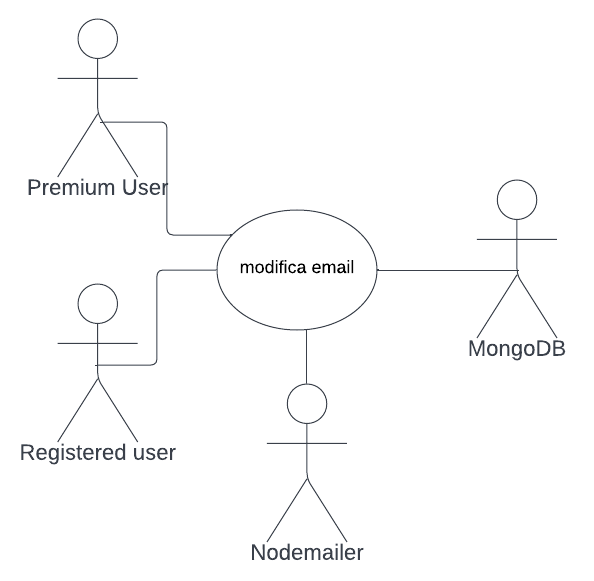
\includegraphics[scale=0.35]{images/use_case_modifica_email.png}
\end{figure}
\noindent
\textbf{Titolo}: modifica e-mail \\
\\
\textbf{Riassunto}: questo use-case spiega come un utente registrato o di livello superiore può modificare la propria e-mail \\
\\
\textbf{Descrizione}:
\begin{enumerate}
    \item L'utente che si trova nella pagina in cui può visualizzare le proprie informazioni personali, decide di modificare la propria e-mail, che è presente in un apposito 'box'. Dopo aver modificato l'e-mail l'utente clicca sul pulsante 'confirm' per confermare la nuova e-mail.
    \item L'applicazione interagisce con il sistema esterno Nodemailer per verificare che l'e-mail inserita sia un e-mail effettivamente esistente e quindi valida. {[ Eccezione 1 ]}
    \item Il sistema interagisce con il database esterno MongoDB per sostituire l'e-mail precedente dell'utente con la nuova e-mail. {[ Eccezione 2 ]}
\end{enumerate}
\textbf{Eccezioni}: \\
{[ Eccezione 1 ]} l'e-mail è inesistente e quindi viene stampato un messaggio di errore all'utente. \\
{[ Eccezione 2 ]} l'e-mail che si è cercato di inserire è gia registrata per un altro account, allora viene stampato a video un messaggio di errore.
\newpage

\subsection{Modifica password} \label{req_modifica_password}

\begin{figure}[!h]
\centering
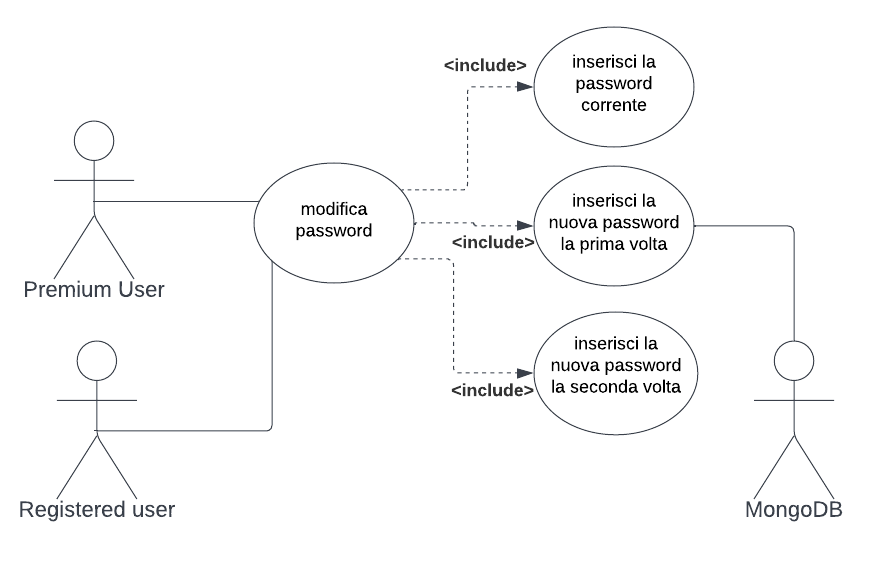
\includegraphics[scale=0.35]{images/use_case_modifica_password.png}
\end{figure}
\noindent
\textbf{Titolo}: modifica password \\
\\
\textbf{Riassunto}: questo use-case spiega come un utente registrato o di livello superiore può modificare la propria password \\
\\
\textbf{Descrizione}:
\begin{enumerate}
    \item L'utente che si trova nella pagina in cui può visualizzare le proprie informazioni personali, decide di modificare la propria password. La modifica della password avviene inserendo in un form: la password precedente, la nuova password una volta e la nuova password una seconda volta. Infine il tutto viene confermato attraverso il pulsante 'confirm'. {[ Eccezione 1 ]}
    \item L'applicazione interagisce con il database esterno MongoDB, il quale modifica la password dell'utente.
\end{enumerate}
\textbf{Eccezioni}: \\
{[ Eccezione 1 ]} alcuni campi sono mancanti oppure i due campi dove viene inserita la nuova password non coincidono e allora viene stampato a video un messaggio di errore.
\newpage

\subsection{Recupero nome utente e password} \label{req_recupero_nome_utente_e_password}
\begin{figure}[!h]
\centering
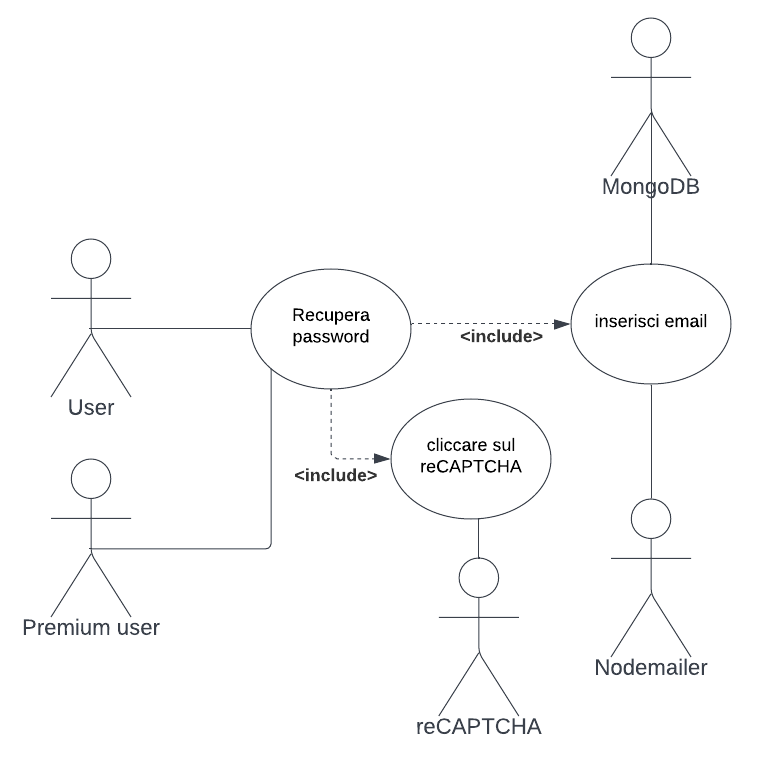
\includegraphics[scale=0.30]{images/use_case_recupero_password.png}
\end{figure}
\noindent
\textbf{Titolo}: recupero username e password \\
\\
\textbf{Riassunto}: questo use-case spiega come un utente registrato o di livello superiore può recuperare la propria password e username, nel caso se li fosse dimenticati \\
\\
\textbf{Descrizione}:
\begin{enumerate}
    \item L'utente che si trova nella pagina di login, clicca sulla scritta 'Forgot password?'. L'applicazione porta l'utente in una pagina dove dovrà inserire la propria e-mail.
    \item Inserita l'e-mail l'utente clicca sul reCAPTCHA e sul pulsante 'Confirm reset password'.
    \item Il sistema genererà una password temporanea, si interfaccia con il database MongoDB, che modificherà la password dell'utente a cui è associata l'e-mail precedentemente inserita. {[ Eccezione 1 ]}
    \item L'applicazione si interfaccerà con il sistema esterno Nodemailer per inviare l'e-mail che conterrà l'username dell'utente con la nuova password.
\end{enumerate}
\textbf{Eccezioni}: \\
{[ Eccezione 1 ]} nel caso in cui non esista nessun utente con associata quella specifica e-mail, viene mostrato un messaggio a video che dice all'utente che l'e-mail inserita non è valida. \\
\newpage

\subsection{Profilo Premium} \label{req_profilo_premium}
\begin{figure}[!h]
\centering
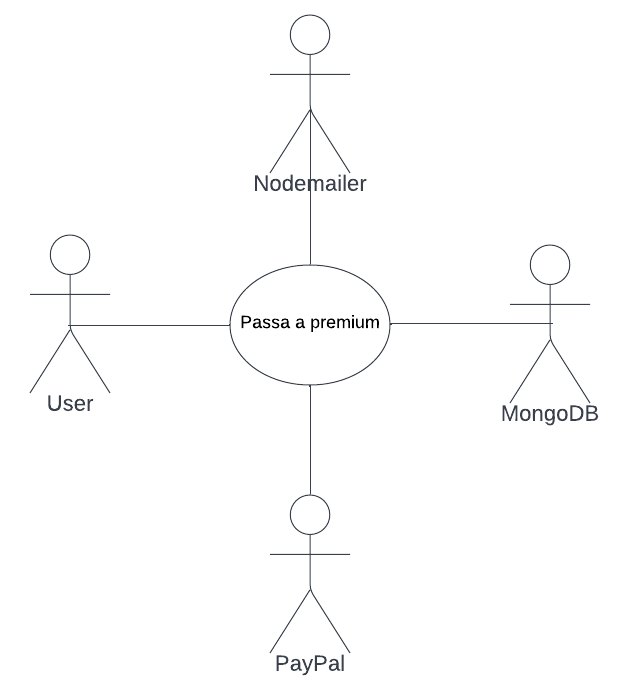
\includegraphics[scale=0.35]{images/use_case_passa_a_premium.png}
\end{figure}
\noindent
\textbf{Titolo}: acquisto versione premium \\
\\
\textbf{Riassunto}: questo use-case spiega come un utente registrato può upgradare il suo profilo a premium. \\
\\
\textbf{Descrizione}:
\begin{enumerate}
    \item L'utente registrato che si trova nella pagina principale dell'applicazione, clicca sul icona del proprio profilo e seleziona la voce 'upgrade profile'.
    \item L'applicazione interagisce con il servizio di pagamento Paypal, con il quale verrà effettuata la transazione di 2.99\euro, all'indirizzo e-mail \href{mailto:lorenzo.dambro@gmail.com}{lorenzo.dambro@gmail.com}.
    \item L'applicazione interagisce con il database MongoDB e aggiorna i privilegi dell'utente, registrandolo come utente premium.
    \item Il sistema invia un e-mail all'utente che lo ringrazia dell'acquisto e che lo avverte che il suo profilo è stato upgradato.
\end{enumerate}
\newpage

\subsection{Quiz tipo 1} \label{req_quiz_1}
\begin{figure}[!h]
\centering
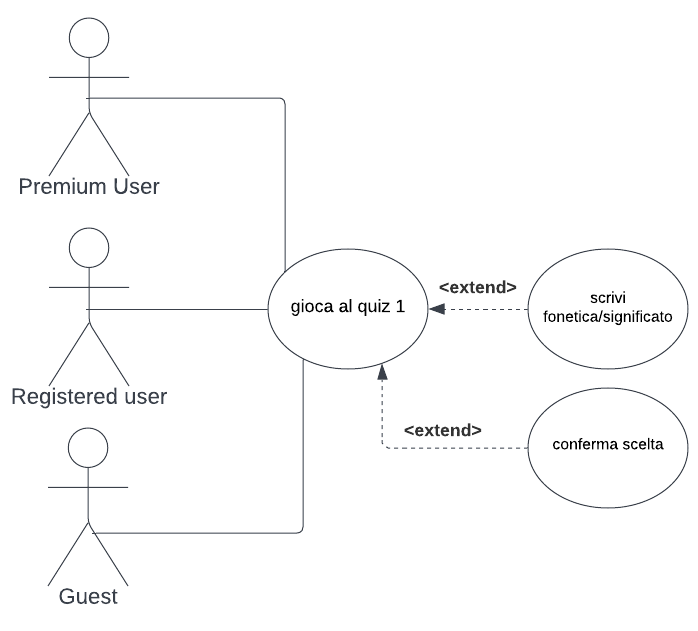
\includegraphics[scale=0.35]{images/use_case_quiz_1.png}
\end{figure}
\noindent
\textbf{Titolo}: Quiz di tipo 1\\
\\
\textbf{Riassunto}: questo use-case spiega come un utente di qualsiasi livello può giocare al quiz di tipo 1.\\
\\
\textbf{Descrizione}:
\begin{enumerate}
    \item L'utente che sta giocando al quiz di tipo 1 si trova davanti al simbolo di uno degli alfabeti scelti dall'utente, ad una casella in cui inserire la fonetica/significato del simbolo e ad un pulsante di conferma, per verificare la correttezza della propria risposta.
    \item L'utente risponde con la fonetica/significato corrispondente, clicca sul pulsante di conferma e il sistema procederà in automatica con la correzione.
    \item L'applicazione rimane in pausa due secondi, per mostrare il risultato della correzione all'utente e poi il sistema procederà con il quiz successivo, oppure tornando alla schermata principale dell'applicazione se non ci sono altri quiz.
\end{enumerate}

\newpage
\subsection{Quiz tipo 2} \label{req_quiz_2}
\begin{figure}[!h]
\centering
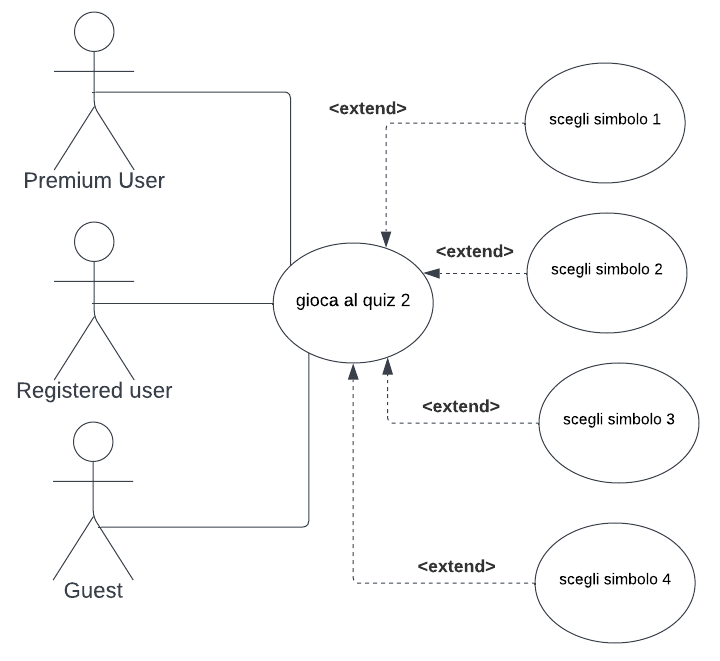
\includegraphics[scale=0.35]{images/use_case_quiz_2.png}
\end{figure}
\noindent
\textbf{Titolo}: Quiz di tipo 2\\
\\
\textbf{Riassunto}: questo use-case spiega come un utente di qualsiasi livello può giocare al quiz di tipo 2.\\
\\
\textbf{Descrizione}:
\begin{enumerate}
    \item L'utente che sta giocando al quiz di tipo 2 si trova davanti alla fonetica/significato di un simbolo di uno degli alfabeti scelti dall'utente e a 4 simboli casuali.
    \item L'utente clicca sul simbolo che è associato alla fonetica/significato corretto.
    \item L'applicazione rimane in pausa due secondi, per mostrare il risultato della correzione all'utente e poi il sistema procederà con il quiz successivo, oppure tornando alla schermata principale dell'applicazione se non ci sono altri quiz.
\end{enumerate}

\newpage
\subsection{Quiz tipo 3} \label{req_quiz_3}
\begin{figure}[!h]
\centering
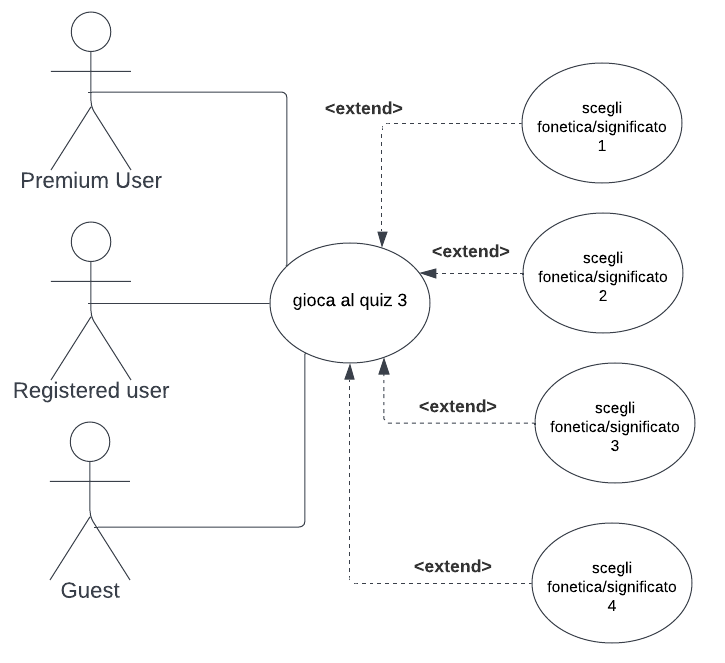
\includegraphics[scale=0.35]{images/use_case_quiz_3.png}
\end{figure}
\noindent
\textbf{Titolo}: Quiz di tipo 3\\
\\
\textbf{Riassunto}: questo use-case spiega come un utente di qualsiasi livello può giocare al quiz di tipo 3.\\
\\
\textbf{Descrizione}:
\begin{enumerate}
    \item L'utente che sta giocando al quiz di tipo 3 si trova davanti ad un simbolo di uno degli alfabeti scelti dall'utente e a 4 fonetiche/significati casuali.
    \item L'utente deve cliccare sulla fonetica/significato che si associa correttamente al simbolo.
    \item L'applicazione rimane in pausa due secondi, per mostrare il risultato della correzione all'utente e poi il sistema procederà con il quiz successivo, oppure tornando alla schermata principale dell'applicazione se non ci sono altri quiz.
\end{enumerate}

\newpage
\subsection{Quiz tipo 4} \label{req_quiz_4}
\begin{figure}[!h]
\centering
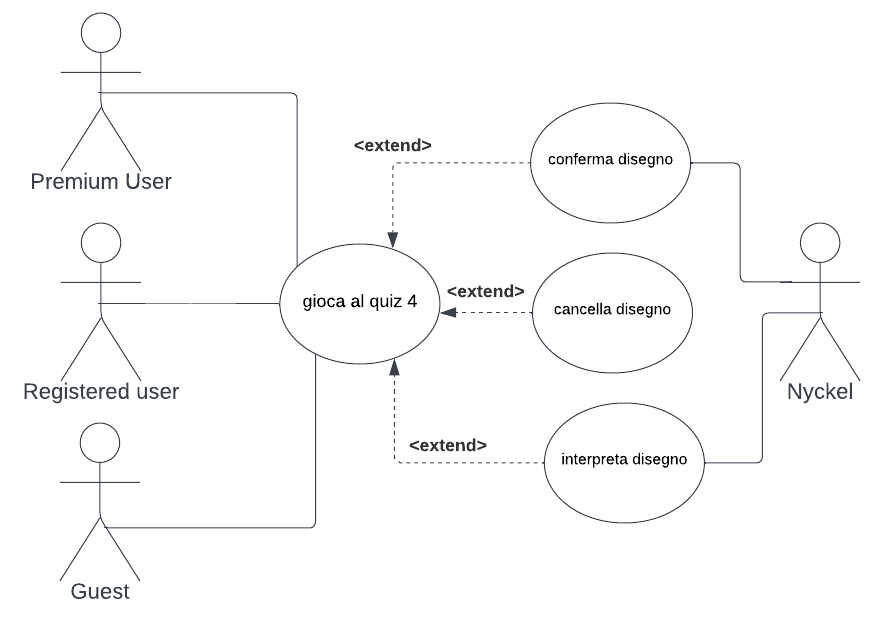
\includegraphics[scale=0.35]{images/use_case_quiz_4.png}
\end{figure}
\noindent
\textbf{Titolo}: Quiz di tipo 4\\
\\
\textbf{Riassunto}: questo use-case spiega come un utente di qualsiasi livello può giocare al quiz di tipo 4.\\
\\
\textbf{Descrizione}:
\begin{enumerate}
    \item L'utente che sta giocando al quiz di tipo 4 si trova davanti alla fonetica/significato (per alfabeti Hirgana e Katakana) o solo al significato (per alfabeti Katakana), ad uno spazio vuoto in cui può disegnare il simbolo e a tre pulsanti 'confirm', 'interpret' e 'cancel'.
    \item L'utente disegna il simbolo a cui è associata la fonetica/significato corrispondente, clicca sul pulsante 'interpret' per verificare che il simbolo sia stato interpretato correttamente dal sistema e infine clicca sul pulsante 'confirm' per confermare quanto disegnato. Quando l'utente clicca sul pulsante 'interpret' o 'confirm' il sistema esterno Nyckel sarà utilizzato per classificare quanto disegnato e quindi per verificare il disegno. Nel caso l'utente volesse ridisegnare il simbolo perchè si rende conto che ha sbagliato oppure il sistema l'ha interpreto in maniera errata allora, può farlo cliccando sul pulsante 'cancel', che cancella quanto precedentemente disegnato.
    \item L'applicazione rimane in pausa due secondi, per mostrare il risultato della correzione all'utente e poi il sistema procederà con il quiz successivo, oppure tornando alla schermata principale dell'applicazione se non ci sono altri quiz.
\end{enumerate}

\newpage
\subsection{Single-player} \label{req_single-player}
\begin{figure}[!h]
\centering
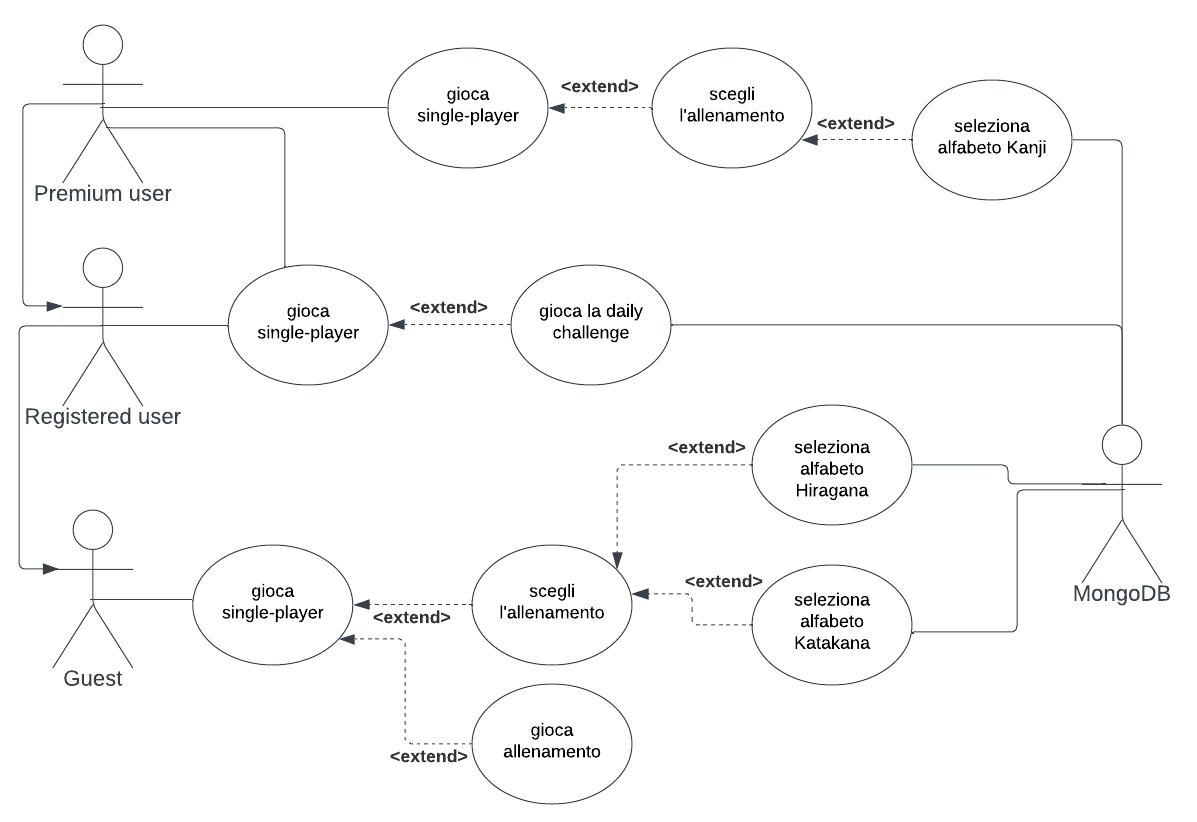
\includegraphics[scale=0.35]{images/use_case_single-player.png}
\end{figure}
\noindent
\textbf{Titolo}: single player \\
\\
\textbf{Riassunto}: questo gruppo di use-case spiega come come l'utente guest o di livello superiore può giocare in modalità single-player.  \\
\\
\textbf{Descrizione}:
\begin{enumerate}
    \item L'utente che si trova nella schermata principale dell'applicazione clicca sul pulsante 'Single-player'.
    \item Si apre una finestra dove l'utente avrà due scelte, effettuare un allenamento con gli alfabeti selezionati cliccando sul pulsante 'Training' oppure provare la sfida giornaliera cliccando sul pulsante 'Daily challenge' (se non l'ha gia effettuata per quello specifico giorno). {[ Eccezione 1 ]}
    \item Effettuate le scelte l'applicazione interagirà con il sistema esterno MongoDB, per riceve la lista dei quiz da proporre all'utente.
    \item A questo punto il gioco inizierà e il sistema porterà l'utente nella pagina dove sarà visualizzato il primo quiz.
\end{enumerate}
{[ Eccezione 1 ]} se l'utente che ha deciso di giocare alla modalità 'training' non ha selezionato nessun alfabeto, allora viene mostrato a video un messaggio di errore, che fa notare all'utente questo problema.

\newpage
\subsection{Multiplayer} \label{req_multiplayer}
\begin{figure}[!h]
\centering
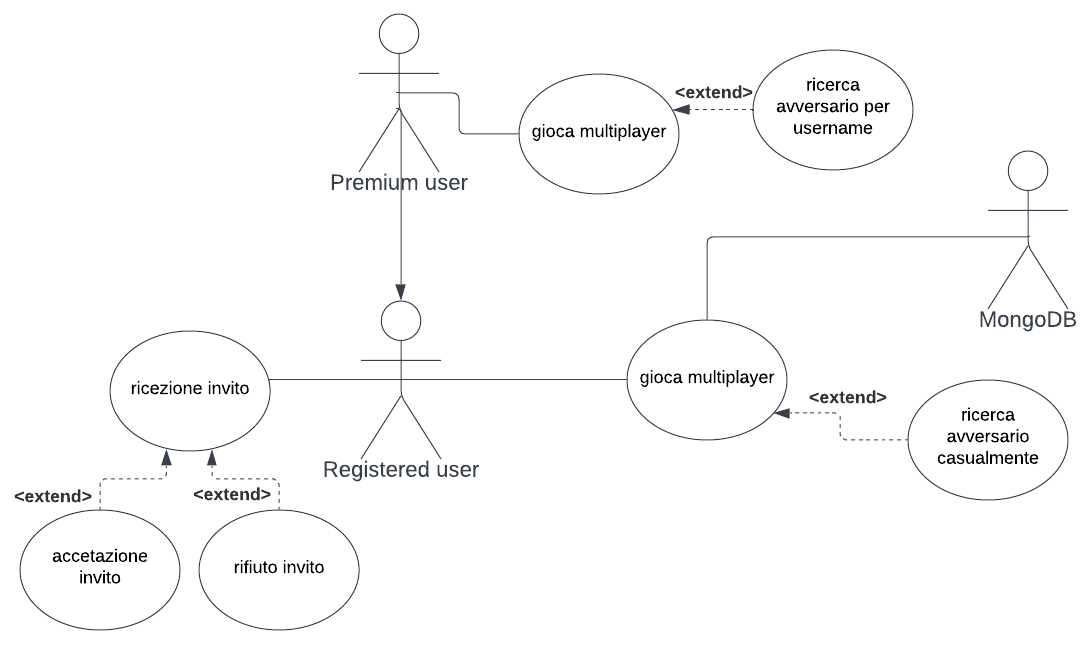
\includegraphics[scale=0.35]{images/use_case_multiplayer.png}
\end{figure}
\noindent
\textbf{Titolo}: multiplayer \\
\\
\textbf{Riassunto}: questo gruppo di use-case spiega come come l'utente registrato o di livello superiore può giocare in modalità multiplayer.  \\
\\
\textbf{Descrizione}:
\begin{enumerate}
    \item L'utente che si trova nella schermata principale dell'applicazione clicca sul pulsante 'Multiplayer'.
    \item Si apre una finestra dove l'utente avrà due scelte, effettuare una ricerca dell'avversario in maniera casuale oppure sfidare un avversario specifico inserendo il suo username.
    \item Effettuata la scelta l'applicazione interagirà con il sistema esterno MongoDB, per riceve la lista dei quiz da proporre ad entrambi gli utenti. {[ Eccezione 1 ]}
    \item Se un utente ha effettuato la ricerca di un avversario per username. L'utente ricercato riceverà una notifica di invito che potrà accettare o rifiutare.
\end{enumerate}
{[ Eccezione 1 ]} se si è ricercato un avversario per username, ma il giocatore ricercato non esiste viene mostrato a video un messaggio di errore.

\newpage
\subsection{Risultato score} \label{req_risultato_score}
\begin{figure}[!h]
\centering
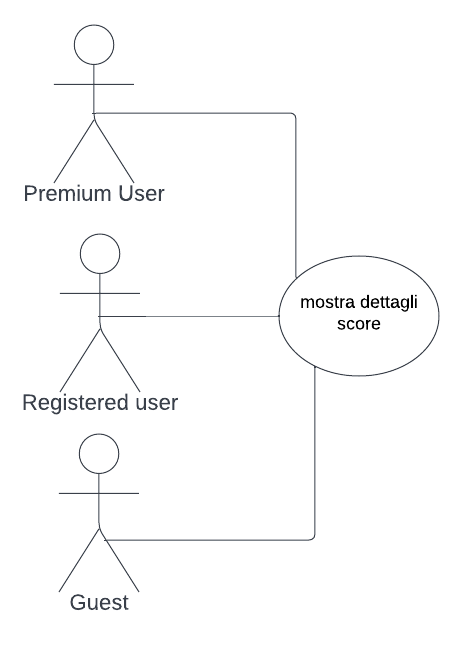
\includegraphics[scale=0.35]{images/use_case_mostra_dettagli_score.png}
\end{figure}
\noindent
\textbf{Titolo}: mostra dettagli score \\
\\
\textbf{Riassunto}: questo use-case spiega come l'utente può visualizzare una serie di informazioni aggiuntive sui quiz fatti, durante una specifica sessione di gioco. \\
\\
\textbf{Descrizione}: 
\begin{enumerate}
    \item L'utente che attualmente si trova nella schermata di uno dei 4 tipi di quiz, clicca sul pulsante 'score' in alto a destra.
    \item Si apre una finestra, in cui compaiono le seguenti informazioni:
    \begin{itemize}
        \item Punteggio totale;
        \item Numero di vittorie, divise tra sfide giornaliere e ranked;
        \item Numero di sconfitte, divise tra sfide giornaliere e ranked;
        \item Rapporto vittorie e sconfitte, divise tra sfide giornaliere e ranked.
    \end{itemize}
\end{enumerate}

\newpage
\subsection{Termina sessione di gioco} \label{req_termina_sessione_gioco}
\begin{figure}[!h]
\centering
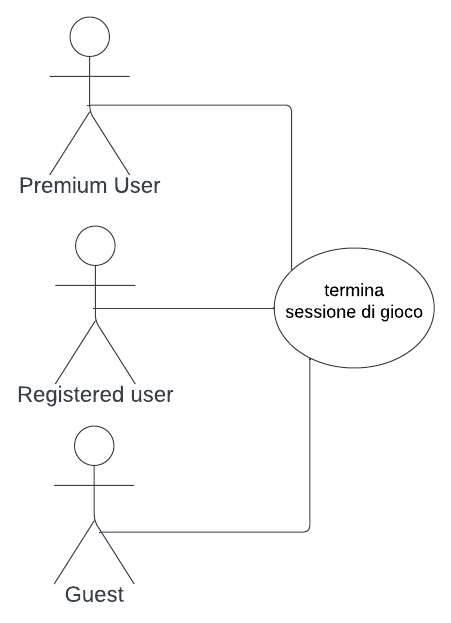
\includegraphics[scale=0.35]{images/use_case_termina_sessione_di_gioco.png}
\end{figure}
\noindent
\textbf{Titolo}: termina sessione di gioco \\
\\
\textbf{Riassunto}: questo use-case spiega come l'utente può terminare la sessione di gioco attuale. \\
\\
\textbf{Descrizione}: 
\begin{enumerate}
    \item L'utente che attualmente si trova nella schermata di uno dei 4 tipi di quiz, clicca sul pulsante 'home' in alto a sinistra.
    \item Il sistema riporta l'utente nella pagina principale dell'applicazione.
\end{enumerate}

\subsection{Visualizzazione statistiche} \label{req_visualizzazione_statistiche}
\begin{figure}[!h]
\centering
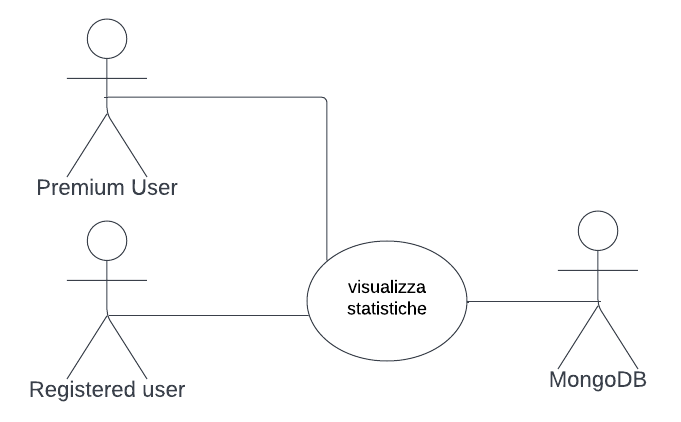
\includegraphics[scale=0.35]{images/use_case_visualizza_statistiche.png}
\end{figure}
\noindent
\textbf{Titolo}: visualizza statistiche \\
\\
\textbf{Riassunto}: questo use-case spiega come un utente registrato o di livello superiore può visualizzare le proprie statistiche personali. \\
\\
\textbf{Descrizione}:
\begin{enumerate}
    \item L'utente che si trova nella pagina principale dell'applicazione, clicca sul icona del proprio profilo e seleziona la voce 'my statistics'.
    \item L'applicazione interagirà con il database esterno MongoDB, per recuperare tutte le statistiche di quello specifico utente e porterà l'utente in una pagina dove potrà visualizzarle. Le statistiche includono: numero partite giocate, punteggio totale, numero di vittorie (giornaliere/ranked), numero di sconfitte (giornaliere/ranked) e rapporto tra vittorie e sconfitte (giornaliere/ranked).
\end{enumerate}

\subsection{Visualizzazione classifica} \label{req_visualizzazione_classifica}
\begin{figure}[!h]
\centering
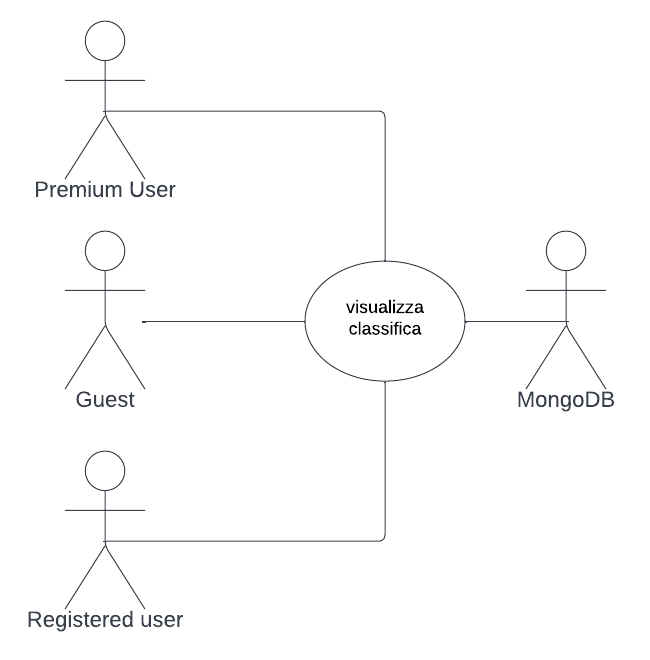
\includegraphics[scale=0.35]{images/use_case_visualizza_classifica.png}
\end{figure}
\noindent
\textbf{Titolo}: visualizzazione classifica \\
\\
\textbf{Riassunto}: questo use-case spiega come un utente di qualsiasi livello può visualizzare la classifica dei giocatori. \\
\textbf{Descrizione}:
\begin{enumerate}
    \item L'utente che si trova nella pagina principale dell'applicazione, clicca sul pulsante "World Ranking".
    \item L'applicazione interagirà con il database esterno MongoDB, per recuperare le informazioni dei primi 100 giocatori e trasferirà l'utente in una nuova pagina, dove gli verrà mostrata la classifica. Le informazioni mostrate saranno: posizione in classifica, nazionalità, username, punteggio totale e partite giocate.
\end{enumerate}

\newpage
\subsection{Ricerca nella classifica} \label{req_ricerca_classifica}
\begin{figure}[!h]
\centering
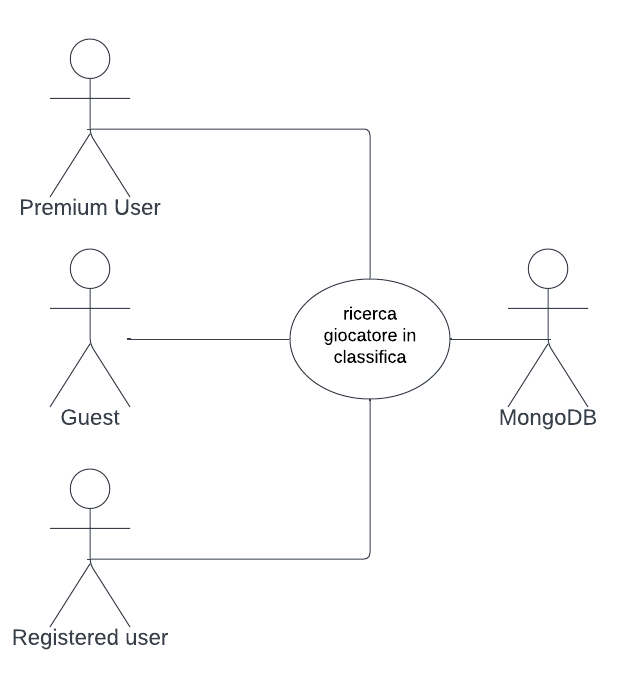
\includegraphics[scale=0.35]{images/use_case_ricerca_giocatore_classifica.png}
\end{figure}
\noindent
\textbf{Titolo}: ricerca nella classifica \\
\\
\textbf{Riassunto}: questo use-case spiega come un utente di qualsiasi livello può effettuare la ricerca di un altro giocatore all'interno della classifica \\
\textbf{Descrizione}:
\begin{enumerate}
    \item L'utente che si trova nella schermata "World Ranking" clicca sulla barra di ricerca e digita il nome del giocatore da ricercare.
    \item L'applicazione interagirà in real time con il database esterno MongoDB per filtrare tutte le statistiche del nome giocatore che l'utente sta digitando.
\end{enumerate}


